% main.tex -- paper source in arXiv format (not submitted to arXiv)
% Build locally with ./build.sh (Tectonic). arXiv recompiles this source with pdfLaTeX
% (TeX Live 2025), so keep the preamble pdfLaTeX-compatible: no fontspec, no \pdfoutput,
% no raw Unicode symbols in the text.
\documentclass[11pt]{article}

% Fonts and encoding
\usepackage[utf8]{inputenc}
\usepackage[T1]{fontenc}
\usepackage{lmodern}
\usepackage{textcomp}
\usepackage{microtype}

% Math, figures, tables, lists, code
\usepackage{amsmath,amssymb,amsfonts}
\usepackage{graphicx}
\usepackage{booktabs}
\usepackage{array}
\usepackage{tabularx}
\usepackage{multirow}
\usepackage{xcolor}
\usepackage{caption}
\usepackage{subcaption}
\usepackage{enumitem}
\usepackage{listings}
\usepackage{tikz}
\usetikzlibrary{arrows.meta,positioning,shapes.geometric,fit,calc}
\usepackage{url}
\usepackage[hidelinks]{hyperref}

% Page geometry
\usepackage[margin=1in]{geometry}

% Allow slight stretch to avoid overfull boxes from long compound terms and URLs
\setlength{\emergencystretch}{2em}

% Table column types that wrap text: L{3cm} left-aligned, C{2cm} centered
\newcolumntype{L}[1]{>{\raggedright\arraybackslash}p{#1}}
\newcolumntype{C}[1]{>{\centering\arraybackslash}p{#1}}

% Code listing style (add language=Python etc. per listing)
\lstdefinestyle{paper}{
  basicstyle=\footnotesize\ttfamily,
  breaklines=true,
  frame=single,
  backgroundcolor=\color{gray!8},
  columns=flexible,
  keepspaces=true,
  showstringspaces=false,
  numbers=left,
  numberstyle=\tiny\color{gray},
  captionpos=b,
}
\lstset{style=paper}

% Paper version: printed under the title and used by ./build.sh release
\newcommand{\paperversion}{0.01}

% Title and authors
\title{The Case for an Objective Score for Open Educational Resources:\\ Proposing the OpenBook QR Score}

\author{
    Dan McCreary \\
    Independent Researcher \\
    \texttt{https://github.com/dmccreary}
}

\date{Version \paperversion \\ \today}

\begin{document}

\maketitle

% Abstract (write it last)
\begin{abstract}
Teachers can find thousands of openly licensed textbooks, but judging whether one is good, and whether it can actually be reused, still rests on opinion. A systematic review of 14 published OER quality rubrics found that five specify no rating scale, only three provide a detailed scoring guide, and only six report any empirical testing. This position paper argues that open educational resources need an objective score: one anchored by descriptors and evidence, reported as separate quality and reusability halves, reproducible by human and AI-agent reviewers, and validated before anyone acts on it. We propose the OpenBook QR Score, ten metrics worth ten points each, five for quality (Q) and five for reusability (R), reported in the form QR 76 (Q 37 / R 39), with a decision rule that stops a high total from hiding a failed metric. As an illustration, not a validation, AI-agent reviewers scored each of ten widely used open textbooks in two independent passes, using about 86,000 tokens and two minutes per title; totals ranged from 60 to 81, and the passes agreed within one point on 88 percent of metric scores. Metadata was the weakest metric (mean 5.5), editable source the strongest (8.9), and eight of ten titles carry a NonCommercial clause that the descriptors do not yet score consistently. Scripted checks on 101 MkDocs book projects apply part of a rubric in seconds per book. We set out the reliability, validity and gaming studies required before scores guide adoption.
\end{abstract}

\noindent\textbf{Keywords:} open educational resources, OER quality, rubric, reusability, AI agents, validation


% Main content sections -- one file per section, in reading order
\section{Introduction}
\label{sec:intro}

Open educational resources (OER) are teaching and learning materials that carry an open license, so that anyone may retain, reuse, revise, remix and redistribute them \cite{wiley5r,wiley2018}. In November 2019 the member states of UNESCO adopted a Recommendation on OER, the first international standard-setting instrument on the topic \cite{unesco2019}. The history of the open-education movement is traced by Weller \cite{weller2014}, and the research literature has been reviewed repeatedly, including for efficacy and user perceptions \cite{wiley2014,hilton2016,hilton2020}, and a recent meta-analysis of 25 studies reports a significant but negligible effect of OER and open educational practices on learning achievement \cite{tlili2023}; whatever their effect on learning, OER matter because they remove cost and permission barriers.

Finding OER is no longer the hard part. Deciding whether a particular resource is good, and whether it can actually be reused in another course, is. A systematic review of OER benefits and challenges lists quality assurance among the main obstacles \cite{adil2022}, and a separate review focuses on the affordability case for OER \cite{mullens2023}. A careful manual review of one textbook takes hours, and two reviewers working from different checklists can reach different conclusions about the same book. The consequence is that adoption decisions rest on opinion, brand recognition or whatever a search engine ranks first.

\paragraph{The gap.}
Rubrics for judging OER exist, but they are not interchangeable. A systematic review of 14 published OER quality rubrics found that five specify no rating scale at all, only three provide a detailed scoring guide, only six report any empirical testing of validity, reliability or utility, and only three were revised several times \cite{yuan2015}. The same review found that the rubrics emphasize different constructs: one focuses on pedagogical value, one on reusability, one on alignment to standards. A reviewer who picks one rubric has implicitly chosen what ``quality'' means. At the same time, generative AI makes it cheap to apply a rubric to a whole catalog, and large language models are already used as judges of text quality \cite{zheng2023,gu2024}. Speed without a validated instrument would simply automate disagreement.

\paragraph{Position.}
This paper argues that the OER ecosystem needs a shared, objective score, and that such a score has to meet four requirements: it must be \emph{anchored} (every level of every metric has a descriptor and every score carries evidence), \emph{two-part} (quality as a learning resource and reusability as a component are reported separately), \emph{reproducible} (the same resource gets the same score from different reviewers, human or machine), and \emph{validated} (the score is tested against reviewer agreement and learner outcomes before anyone acts on it). ``Objective'' is used here in the measurement sense of inter-subjective and checkable, not in the sense of free of judgment; Section~\ref{sec:requirements} makes this precise.

\paragraph{Contributions.}
We make five contributions.
\begin{enumerate}[leftmargin=*,itemsep=2pt]
  \item We argue for four requirements that an OER score must meet and show, using the published review of rubrics, which of them current practice meets (Section~\ref{sec:requirements}).
  \item We propose the \emph{OpenBook QR Score}, a 100-point instrument made of ten metrics worth ten points each, five for quality (Q) and five for reusability (R), with a fixed reporting format and decision rule (Section~\ref{sec:score}). We specify it fully enough to be applied or rebutted.
  \item We illustrate the instrument on ten widely used open textbooks, each scored in two independent passes by AI-agent reviewers (one sampled chapter, then three), and report the scores, the agreement between passes, the elapsed time and the token cost. We also report 13 scripted checks run on 101 MkDocs book projects (Section~\ref{sec:illustration}). This evidence comes from one model family and is unvalidated; we use it to show what the instrument surfaces and where it is weak, not to rank the books.
  \item We identify specific under-specifications that the illustration exposes, notably how a NonCommercial license should affect the license metric.
  \item We state a validation agenda: the studies required before QR scores are used to make adoption decisions (Section~\ref{sec:validation}).
\end{enumerate}

\paragraph{Roadmap.}
Section~\ref{sec:related} reviews four strands of prior work. Section~\ref{sec:requirements} states the requirements. Section~\ref{sec:score} specifies the score. Section~\ref{sec:illustration} applies it. Section~\ref{sec:validation} sets out the validation agenda, Section~\ref{sec:discussion} discusses implications and limitations, Section~\ref{sec:nextstep} describes the next step, and Section~\ref{sec:conclusion} concludes. Throughout, the work is a fast, low-cost first step, not a validation.

\section{Background and Related Work}
\label{sec:related}

\subsection{Rubrics for OER quality}
The most direct prior work is the review of 14 OER quality rubrics by Yuan and Recker \cite{yuan2015}. It examined them along content, development process and application context, and found wide diversity: the number of indicators ranges from 3 to 42, five rubrics specify no rating scale, only three give a detailed scoring guide, only six report empirical testing and two target automated evaluation. The Learning Object Review Instrument (LORI) stands out in that review for combining a rating scale, a scoring guide, reported testing and several revisions. Other work asks users what they want. Clements and Pawlowski surveyed teachers who use OER repositories about how they re-use resources and perceive quality, and report that trust in resources, organizations and technologies matters in particular \cite{clements2012}. Bliss and colleagues studied college teacher and student perceptions of OER \cite{bliss2013}. A recent systematic review still lists quality assurance as a challenge \cite{adil2022}, and a meta-synthesis of the literature on open education practices shows how broadly the field is defined \cite{shareefa2023}. \emph{This paper differs} by taking the review's findings as requirements: a score must have a scale, anchors and evidence, and it must be tested before it is trusted.

\subsection{Reusability and metadata}
Reuse is a separate construct from teaching quality, yet rubrics mostly fold it in as one indicator or one emphasis. Work on learning objects proposed automatic metrics for the quality of metadata in digital repositories \cite{ochoa2009} and relevance-ranking metrics for learning objects \cite{ochoa2008}. In scientific data, the FAIR principles make findability, accessibility, interoperability and reusability explicit, machine-checkable properties \cite{wilkinson2016}. Openness itself has a defined set of permissions \cite{wiley5r,wiley2018}, and accessibility has a published standard \cite{wcag21}. \emph{This paper differs} by treating reusability as a co-equal half of the score, with its own five metrics, so that a resource can be shown to be strong in one half and weak in the other.

\subsection{Validity, reliability and rubric use}
A score is only as good as the argument that supports its use. Messick and Kane describe validation as building and testing an interpretation-and-use argument \cite{messick1995,kane2013}. Reviews of rubric research find that analytic rubrics with explicit descriptors can support consistent scoring, but evidence about validity is thinner than evidence about reliability \cite{jonsson2007,reddy2010}. Agreement between raters is reported with Cohen's kappa \cite{cohen1960}, intraclass correlation \cite{shrout1979,koo2016} and chance-corrected coefficients that behave better when agreement is high \cite{gwet2008}, interpreted with conventional benchmarks \cite{landis1977}. Measurement also changes behavior: once a metric becomes a target it stops being a good measure \cite{campbell1979,strathern1997}. \emph{This paper differs} by naming these methods as the required validation program for an OER score, and by flagging gaming as a design risk.

\subsection{AI agents as evaluators}
Large language models are used to grade and rate text, and agreement with humans can be high enough to be useful but is affected by position and verbosity biases \cite{zheng2023,wang2024}. Prompted judges that follow criteria align better with humans on some tasks \cite{liu2023}, and a survey catalogs strategies for making judges reliable \cite{gu2024}. Models also produce confident falsehoods, including fabricated citations \cite{ji2023}, and carry risks when used in education \cite{bender2021,kasneci2023,zawacki2019}. In education, one study compared crowdsourced and language-model-based applications of two standardized rubrics to 30 assessment items across six domains \cite{moore2024}, and the open-education community has begun to examine how generative AI relates to OER and open educational practices \cite{bozkurt2023}. \emph{This paper differs} by treating the agent as one possible reviewer inside a score whose validity is established separately, rather than as the source of the score's authority.

\section{Why OER Need an Objective Score}
\label{sec:requirements}

\subsection{What ``objective'' can mean for a rubric}
No score of educational material is free of judgment. We use ``objective'' in the sense used in measurement: a score is objective to the degree that trained reviewers, working independently from the same stated criteria and evidence, arrive at the same number. This is a property that can be measured and reported, for example as a chance-corrected agreement coefficient \cite{cohen1960,gwet2008} or an intraclass correlation \cite{shrout1979,koo2016}. It is also a property that is lost without effort: a vague descriptor, an unrecorded source or a reviewer's preference for a familiar publisher all move a score without moving the resource. An objective score therefore needs more than a list of criteria. It needs rules that tie each number to evidence.

\subsection{Four requirements}
We propose four requirements for an OER score meant to inform adoption decisions. Table~\ref{tab:requirements} sets each beside what the published review of OER rubrics found \cite{yuan2015}.

\begin{table}[htbp]
\centering
\caption{Four requirements for an objective OER score and what the review of 14 published rubrics \cite{yuan2015} reports for each. Counts are numbers of rubrics out of 14.}
\label{tab:requirements}
\small
\begin{tabular}{@{}L{2.6cm}L{5.2cm}L{6.4cm}@{}}
\toprule
Requirement & What it means & Evidence from the review of 14 rubrics \\
\midrule
R1 Anchored & Every level of every metric has a descriptor, and every score cites evidence. & 5 specify no rating scale; only 3 provide a detailed scoring guide. \\
R2 Two-part & Quality as a learning resource and reusability as a component are scored and reported separately. & Rubrics emphasize different constructs (pedagogy, reusability, standards alignment). One rubric lists reusability as one of nine indicators. \\
R3 Reproducible & Different reviewers, human or AI agent, reach the same score, and each step can be audited. & Only 2 target automated evaluation. \\
R4 Validated & The score is tested for reliability, validity and utility before it guides decisions, and is revised as evidence arrives. & Only 6 report empirical testing; only 3 were revised several times. \\
\bottomrule
\end{tabular}
\end{table}

\paragraph{R1: Anchored.}
Anchoring is what turns a checklist into a measurement. If a reviewer's 7 and another's 9 cannot be compared, totals cannot be compared either. Descriptors tie each level to the share of a metric's checks that a resource meets, and an evidence rule makes a score auditable: a reviewer, or an agent, must say where in the resource each number came from.

\paragraph{R2: Two-part.}
A resource can teach well and still be impossible to reuse, for example an excellent text distributed only as a PDF under a restrictive license. It can also be perfectly open and weak. These are different problems with different remedies, and a single blended number hides which one a resource has. The score must therefore keep the halves visible in its reporting format, not only in an appendix.

\paragraph{R3: Reproducible, by humans and by agents.}
Applying a rubric to a catalog of thousands of resources is a task for software. Some checks, such as whether a license is stated, whether images have alternative text, or whether source files are published, can be scripted and are exactly repeatable. Others, such as whether facts are accurate or practice matches outcomes, need judgment, and an AI agent can make a first pass. Agents also invent citations, misread licenses and report more confidence than their evidence supports \cite{ji2023,zheng2023,wang2024}. Reproducibility therefore requires separating scripted checks from judgment, recording evidence for each, and measuring agent agreement with humans rather than assuming it.

\paragraph{R4: Validated.}
Validation is an argument about the interpretation and use of a score, supported by evidence \cite{messick1995,kane2013}. For an adoption score the central claims are that reviewers agree, that scores track the properties they name, and that using scores leads to better adoption decisions. A score published before this evidence exists should say so, label its numbers provisional and invite correction.

\subsection{Why now}
Two developments raise the stakes. First, the supply of openly licensed material keeps growing under policy support \cite{unesco2019}, so the cost of unstructured review grows with it. Second, language-model agents make it practical to score a whole catalog in minutes. Section~\ref{sec:illustration} reports what that cost in one illustration. Cheap scoring is an opportunity only if the score is trustworthy; otherwise it multiplies unvalidated numbers, and once a number becomes a target it is likely to be gamed \cite{campbell1979,strathern1997}.

\subsection{What an objective score does not claim}
A rubric examines a resource, not its results. A high score does not show that students learn more from the resource, and it does not replace the instructor's judgment about fit with a particular course. The relationship between rubric scores and learner outcomes is an empirical question, and the proposal treats it as one (Section~\ref{sec:validation}).

\section{The OpenBook QR Score}
\label{sec:score}

This section specifies the instrument. The name expresses its structure: QR is \emph{Quality} plus \emph{Reusability}, out of 100. The specification is the one taught in an open intelligent textbook on OER evaluation \cite{oerevaluator}; Figure~\ref{fig:workflow} shows how a score is produced and checked.

\begin{figure}[htbp]
  \centering
  \resizebox{\linewidth}{!}{% TikZ figure: how an OpenBook QR Score is produced and checked.
% Explicit coordinates keep every box clear of the others; the figure is scaled to the text width in the section file.
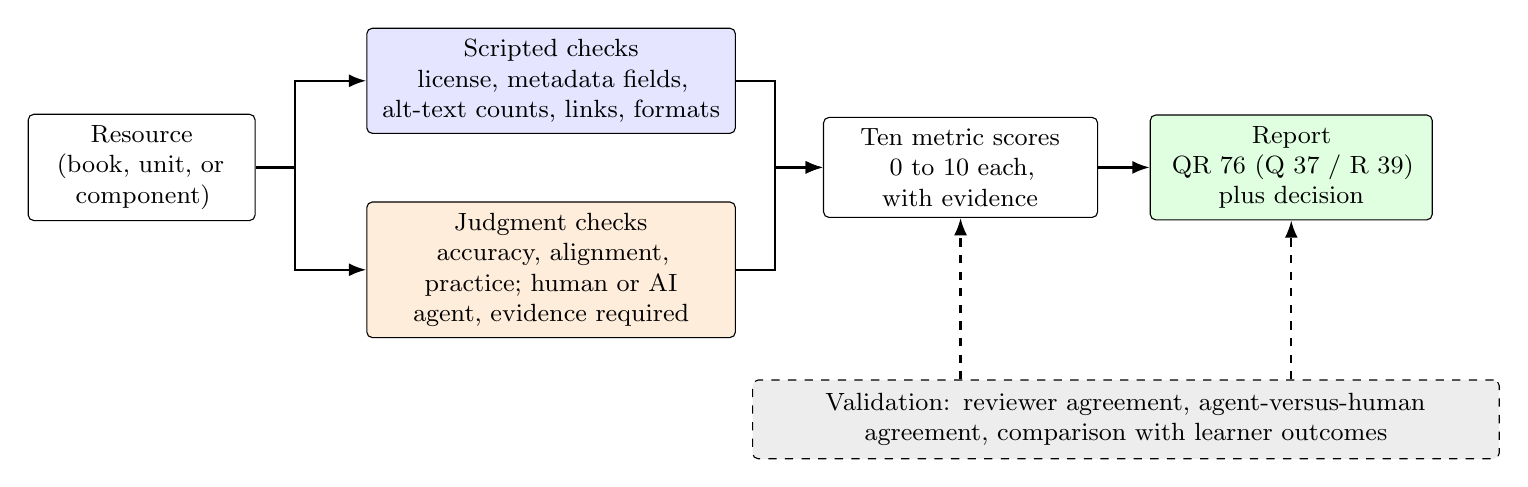
\begin{tikzpicture}[
  box/.style={draw, rounded corners=2pt, align=center, minimum height=10mm, font=\small, inner sep=4pt},
  det/.style={box, fill=blue!10, text width=4.4cm},
  jud/.style={box, fill=orange!14, text width=4.4cm},
  ten/.style={box, text width=3.2cm},
  outc/.style={box, fill=green!12, text width=3.3cm},
  chk/.style={box, fill=gray!14, dashed, text width=9.2cm},
  arr/.style={-{Latex[length=2.2mm]}, thick}
]
\node[box, text width=2.6cm] (res) at (0,0) {Resource\\(book, unit, or component)};
\node[det] (det) at (5.2,1.1) {Scripted checks\\license, metadata fields, alt-text counts, links, formats};
\node[jud] (jud) at (5.2,-1.3) {Judgment checks\\accuracy, alignment, practice; human or AI agent, evidence required};
\node[ten] (ten) at (10.4,0) {Ten metric scores\\0 to 10 each,\\with evidence};
\node[outc] (qr) at (14.6,0) {Report\\QR 76 (Q 37 / R 39)\\plus decision};
\node[chk] (val) at (12.5,-3.2) {Validation: reviewer agreement, agent-versus-human agreement, comparison with learner outcomes};
\draw[arr] (res.east) -- ++(0.5,0) |- (det.west);
\draw[arr] (res.east) -- ++(0.5,0) |- (jud.west);
\draw[arr] (det.east) -- ++(0.5,0) |- (ten.west);
\draw[arr] (jud.east) -- ++(0.5,0) |- (ten.west);
\draw[arr] (ten) -- (qr);
\draw[arr, dashed] (val.north -| ten.south) -- (ten.south);
\draw[arr, dashed] (val.north -| qr.south) -- (qr.south);
\end{tikzpicture}
}
  \caption{How an OpenBook QR Score is produced. A resource passes through scripted checks (blue) and judgment checks (orange) that yield ten metric scores with evidence, which are summed into a report such as QR 76 (Q 37 / R 39) and a decision. Validation studies (gray, dashed) test the scores and feed back into the metrics and descriptors.}
  \label{fig:workflow}
\end{figure}

\subsection{Unit of evaluation}
The unit is a \emph{resource}: a whole textbook, a chapter, or a reusable component such as a quiz or an interactive simulation. Every score names the unit, the version evaluated and the date, because resources change and a score describes the resource as it stood.

\subsection{The ten metrics}
The score has ten metrics worth ten points each. Five measure quality (Q) and five measure reusability (R). Table~\ref{tab:metrics} lists them with the question each answers and the evidence a reviewer collects. The last column marks how far each is open to scripting; this is a design proposal that the validation program should test, not a finding.

\begin{table}[htbp]
\centering
\caption{The ten metrics of the OpenBook QR Score. ``Scripting'' marks how much of the metric can be checked mechanically (high, partial, low); the remainder needs human or agent judgment.}
\label{tab:metrics}
\small
\begin{tabular}{@{}rL{2.6cm}L{6.3cm}C{1.4cm}@{}}
\toprule
\# & Metric & What is checked & Scripting \\
\midrule
\multicolumn{4}{@{}l}{\textit{Quality (Q)}} \\
1 & Accuracy and currency & Facts match cited sources; sources and data are current; edition date and corrections process stated. & low \\
2 & Alignment & Sections map to stated learning outcomes; activities and tests match them; a range of Bloom levels. & partial \\
3 & Readability & Reading level fits the audience; terms are defined before use. & partial \\
4 & Accessibility & Alternative text, heading structure, captions, contrast, conformance with WCAG 2.1 AA \cite{wcag21}. & partial \\
5 & Practice with feedback & Exercises, worked examples, quizzes or simulations that tell learners how they did. & partial \\
\addlinespace
\multicolumn{4}{@{}l}{\textit{Reusability (R)}} \\
6 & Open license & A clear license is stated on the work and its parts; version, owner and attribution are given. & high \\
7 & Modularity & Each section, quiz or simulation stands alone and can be embedded elsewhere. & partial \\
8 & Metadata & Title, author, subject, level, license and description are recorded in a machine-readable form. & high \\
9 & Editable source & Source is published in an editable open format, not only as a fixed document. & high \\
10 & Portability & The resource works elsewhere without a login: downloadable formats, embeddable by link. & partial \\
\bottomrule
\end{tabular}
\end{table}

\subsection{Scale and descriptors}
Each metric is scored with a whole number from 0 to 10. Whole numbers are deliberate: half points suggest a precision human reviewers cannot deliver. A reviewer counts the checks the resource meets, finds the share $p$ of applicable checks met, and chooses the band in Table~\ref{tab:bands}. Within a two-number band the reviewer picks the lower number if a gap would stop a learner or a reuser from doing what the check protects, and the higher if the gaps are cosmetic. A 10 requires that every check pass everywhere it applies.

\begin{table}[htbp]
\centering
\caption{Scoring descriptors. Every metric uses the same scale, so a 6 for readability and a 6 for portability both mean that roughly half to three quarters of the check is in place.}
\label{tab:bands}
\small
\begin{tabular}{@{}cL{2.2cm}L{6.5cm}C{2.4cm}@{}}
\toprule
Score & Descriptor & What it looks like & Share of check met \\
\midrule
0 & Absent & The resource fails the check completely. & 0\% \\
1--2 & Very poor & A token effort is present; most of the check is unmet. & 1--24\% \\
3--4 & Weak & Some of the check is met; gaps would stop many learners or reusers. & 25--49\% \\
5--6 & Adequate & About half to three quarters met, with clear gaps. & 50--74\% \\
7--8 & Good & Most of the check is met, with minor gaps. & 75--89\% \\
9--10 & Excellent & Nearly all or all of the check is met. & 90--100\% \\
\bottomrule
\end{tabular}
\end{table}

Four rules keep scores honest. \emph{Score what you checked}: a reviewer who did not test the embed cannot score portability. \emph{Score the resource as it is today}, not a promised fix. \emph{Score each metric by itself}, so strength on one metric does not lift another. \emph{Record a number for every metric}, with its evidence; when something cannot be determined, record it as unverified and score conservatively from what was verified.

\subsection{Aggregation, report and decision rule}
Let $s_i \in \{0,\dots,10\}$ be the score for metric $i$. The subtotals and total are
\begin{equation}
  Q = \sum_{i=1}^{5} s_i, \qquad R = \sum_{i=6}^{10} s_i, \qquad T = Q + R .
  \label{eq:total}
\end{equation}
The report always gives all three numbers, in the form \texttt{QR $T$ (Q $Q$ / R $R$)}. For example, a resource with $Q=37$ and $R=39$ is reported as ``QR 76 (Q 37 / R 39)''. Totals fall in five bands: excellent (90--100), good (75--89), fair (50--74), weak (25--49) and poor (0--24). The proposed decision rule for an adopter, with $m=\min_i s_i$, is
\begin{equation}
  \text{decision} =
  \begin{cases}
    \text{Adopt}  & T \ge 75 \text{ and } m \ge 5,\\
    \text{Reject} & T < 50,\\
    \text{Revise} & \text{otherwise.}
  \end{cases}
  \label{eq:decision}
\end{equation}
The floor $m \ge 5$ prevents a strong total from hiding a failed metric.

\subsection{Design decisions and rejected alternatives}
\paragraph{Equal weights.} Every metric carries ten points. We know of no evidence that would justify unequal weights, and weights would add parameters that need validation of their own. Weights can be learned later from outcome data.

\paragraph{Two halves, one total.} Reporting only a total would hide the quality-versus-reusability split that motivates the score (R2). Reporting only two numbers would make comparison across hundreds of resources awkward. The format keeps both. The companion component-level specification \cite{oerevaluator} deliberately never blends its two headline numbers, so whether a combined total should be reported at all remains open (Section~\ref{sec:discussion}).

\paragraph{Ten metrics.} The review reports indicator counts from 3 to 42 across rubrics (mean 15.5) and notes that more indicators burden the people who apply them \cite{yuan2015}. Ten metrics cover both halves while staying short enough for a careful reviewer to finish; the five-and-five split follows from R2 rather than from evidence about the right number of metrics.

\paragraph{Whole-number scale with descriptors.} Binary scales discard information; five-point scales offer too little resolution for totals; continuous scales invite false precision. Eleven levels grouped into six described bands are a compromise that descriptors can anchor.

\paragraph{Scripted versus judged.} Checks that can be scripted (license present, metadata fields, image alternative text, published source) are scripted, because scripts are exactly repeatable. Judgment checks are made by humans or agents and must cite evidence. Keeping the two apart lets the validation program study agent error where it matters, in the judgment checks.

\section{Illustration: Applying the Score to Ten Open Textbooks}
\label{sec:illustration}

This section applies the specification to real resources. It is an \emph{illustration}, not a validation: every score was produced by an AI agent from the same model family, and no human reviewer scored the same resources. Its purposes are to show that the instrument can be applied at low cost, to show what it surfaces, to measure how stable the scores are across two independent passes, and to expose where the specification is too loose.

\subsection{Method}
\paragraph{Selection.}
No public title-level ranking of OER popularity exists that we could find, so ``widely used'' is a judgment. We chose six OpenStax titles (College Physics 2e, Biology 2e, Psychology 2e, Principles of Economics 3e, Calculus Volume 1, Anatomy and Physiology 2e) and four titles from other publishers (OpenIntro Statistics; \emph{A First Course in Linear Algebra} by Beezer; \emph{Think Python}; \emph{Eloquent JavaScript}) to span subjects, publishers and source formats. This is a convenience sample, not a random one, and it over-represents one publisher.

\paragraph{Two passes.}
All ten titles were scored twice on 31 October 2026, by separate agents that did not see each other's scores. Each agent received an identical brief containing the ten metrics, the descriptors of Table~\ref{tab:bands}, the four scoring rules and the decision rule of Equation~\ref{eq:decision}. Agents used web search, page and API fetches and small scripts, and they ran on the default subagent model, which inherits the session's model (Claude Sonnet 5.5).
\begin{itemize}[leftmargin=*,itemsep=2pt]
  \item \emph{First pass (one chapter).} Metrics 1 to 5 were scored from front matter and the fifth chapter in the table of contents; metrics 6 to 10 from the whole work.
  \item \emph{Second pass (three chapters).} We changed the sampling after noticing that one chapter is a thin basis for the quality metrics. Metrics 1 to 5 were scored separately for the first, middle and last numbered chapters, and the reported score is the mean rounded half up. Metrics 6 to 10 were again scored from the whole work. Agents worked in their own folders.
\end{itemize}
Each agent returned a record with the scores, one or two sentences of located evidence per metric, a self-reported confidence per metric, a list of what it could not verify, a Flesch--Kincaid grade for each sampled chapter and image alternative-text counts. Unless stated otherwise, the results below are from the second pass; the first pass is used for the comparison in Section~\ref{sec:retest}.

\paragraph{Scripted census.}
Separately, we ran the 13 scripted book-level completeness checks of a companion evaluator skill \cite{oerevaluator} on MkDocs book projects in the author's workspace. The checks are static analysis of files on disk: license, creators, sponsor, objectives, learners, prerequisites, instructions, accessibility mention, technical requirements, references, internal links, practice questions and image alternative text.

\emph{How the 101 were chosen.} Selection was by file layout, not by content. The workspace has 160 top-level folders; 143 contain a \texttt{mkdocs.yml}; 111 of those also have a \texttt{docs/chapters} folder; and the 101 with at least five entries there form the census. The threshold of five was fixed before the run to skip scaffolds and stubs and was not tuned against results; a threshold of one would admit 111. Because the rule looks only at layout, the 101 are not all textbooks. They include repositories that appear from their names to be tooling, documentation or hardware projects (for example a repository of agent skills and a catalog of simulations), and they include the companion book from which the rubric comes. We did not classify them by hand; Section~\ref{sec:census} reports the effect of excluding the obvious candidates.

\emph{Which versions.} Before the run we updated every one of the 111 candidates on 31 October 2026 with \texttt{git pull --ff-only}, which fast-forwards or refuses and never merges. Of the 101 census books, 76 were already current, 6 fast-forwarded, and 19 refused: 11 have histories that diverge from their remote, 5 contain unresolved merge conflicts, and 3 have local edits that the update would overwrite. Refused books were inspected as they stand locally. The checks read the working tree, not a commit, so the 40 books with uncommitted edits were inspected with those edits. The commit, dirty state and pull outcome of every book are recorded with the data.

\subsection{Scores of ten textbooks}
Table~\ref{tab:scores} gives the second-pass results. Totals range from 60 to 81 (mean 72.9, median 77.5). Six titles meet the Adopt rule of Equation~\ref{eq:decision}, all from OpenStax; none reaches the excellent band, and the four titles from other publishers all land in Revise. Figure~\ref{fig:qr} plots Q against R, and Figure~\ref{fig:profile} shows each metric's mean and range.

\begin{table}[htbp]
\centering
\caption{OpenBook QR Scores for ten open textbooks from the three-chapter pass, sorted by total. Metric scores are $s_1$ to $s_{10}$ in the order of Table~\ref{tab:metrics}. $T_1$ is the total from the independent one-chapter pass. Scores are provisional and unvalidated: one AI-agent reviewer per title per pass.}
\label{tab:scores}
\scriptsize
\setlength{\tabcolsep}{3.0pt}
\begin{tabular}{@{}lccccccccccccccc@{}}
\toprule
Title & $s_1$ & $s_2$ & $s_3$ & $s_4$ & $s_5$ & $s_6$ & $s_7$ & $s_8$ & $s_9$ & $s_{10}$ & Q & R & T & $T_1$ & Decision \\
\midrule
OpenStax Physics 2e & 8 & 8 & 8 & 8 & 8 & 8 & 9 & 7 & 9 & 8 & 40 & 41 & 81 & 79 & Adopt \\
OpenStax Calculus 1 & 8 & 8 & 8 & 8 & 8 & 9 & 8 & 7 & 9 & 8 & 40 & 41 & 81 & 73 & Adopt \\
OpenStax Anat.\ \& Phys.\ 2e & 8 & 8 & 8 & 8 & 6 & 8 & 9 & 8 & 9 & 8 & 38 & 42 & 80 & 80 & Adopt \\
OpenStax Economics 3e & 7 & 8 & 8 & 8 & 7 & 9 & 8 & 8 & 9 & 8 & 38 & 42 & 80 & 83 & Adopt \\
OpenStax Psychology 2e & 7 & 8 & 8 & 8 & 6 & 9 & 8 & 7 & 9 & 8 & 37 & 41 & 78 & 76 & Adopt \\
OpenStax Biology 2e & 8 & 8 & 7 & 8 & 5 & 8 & 9 & 7 & 9 & 8 & 36 & 41 & 77 & 76 & Adopt \\
Think Python 3e & 8 & 5 & 8 & 5 & 6 & 7 & 8 & 4 & 10 & 6 & 32 & 35 & 67 & 69 & Revise \\
OpenIntro Statistics & 8 & 6 & 7 & 3 & 8 & 8 & 5 & 3 & 9 & 7 & 32 & 32 & 64 & 73 & Revise \\
Eloquent JavaScript 4e & 8 & 3 & 7 & 6 & 5 & 6 & 8 & 2 & 8 & 8 & 29 & 32 & 61 & 68 & Revise \\
Beezer Linear Algebra & 6 & 4 & 8 & 3 & 8 & 7 & 7 & 2 & 8 & 7 & 29 & 31 & 60 & 59 & Revise \\
\midrule
Mean (all ten) & 7.6 & 6.6 & 7.7 & 6.5 & 6.7 & 7.9 & 7.9 & 5.5 & 8.9 & 7.6 & 35.1 & 37.8 & 72.9 & 73.6 & \\
\bottomrule
\end{tabular}
\end{table}

\begin{figure}[htbp]
  \centering
  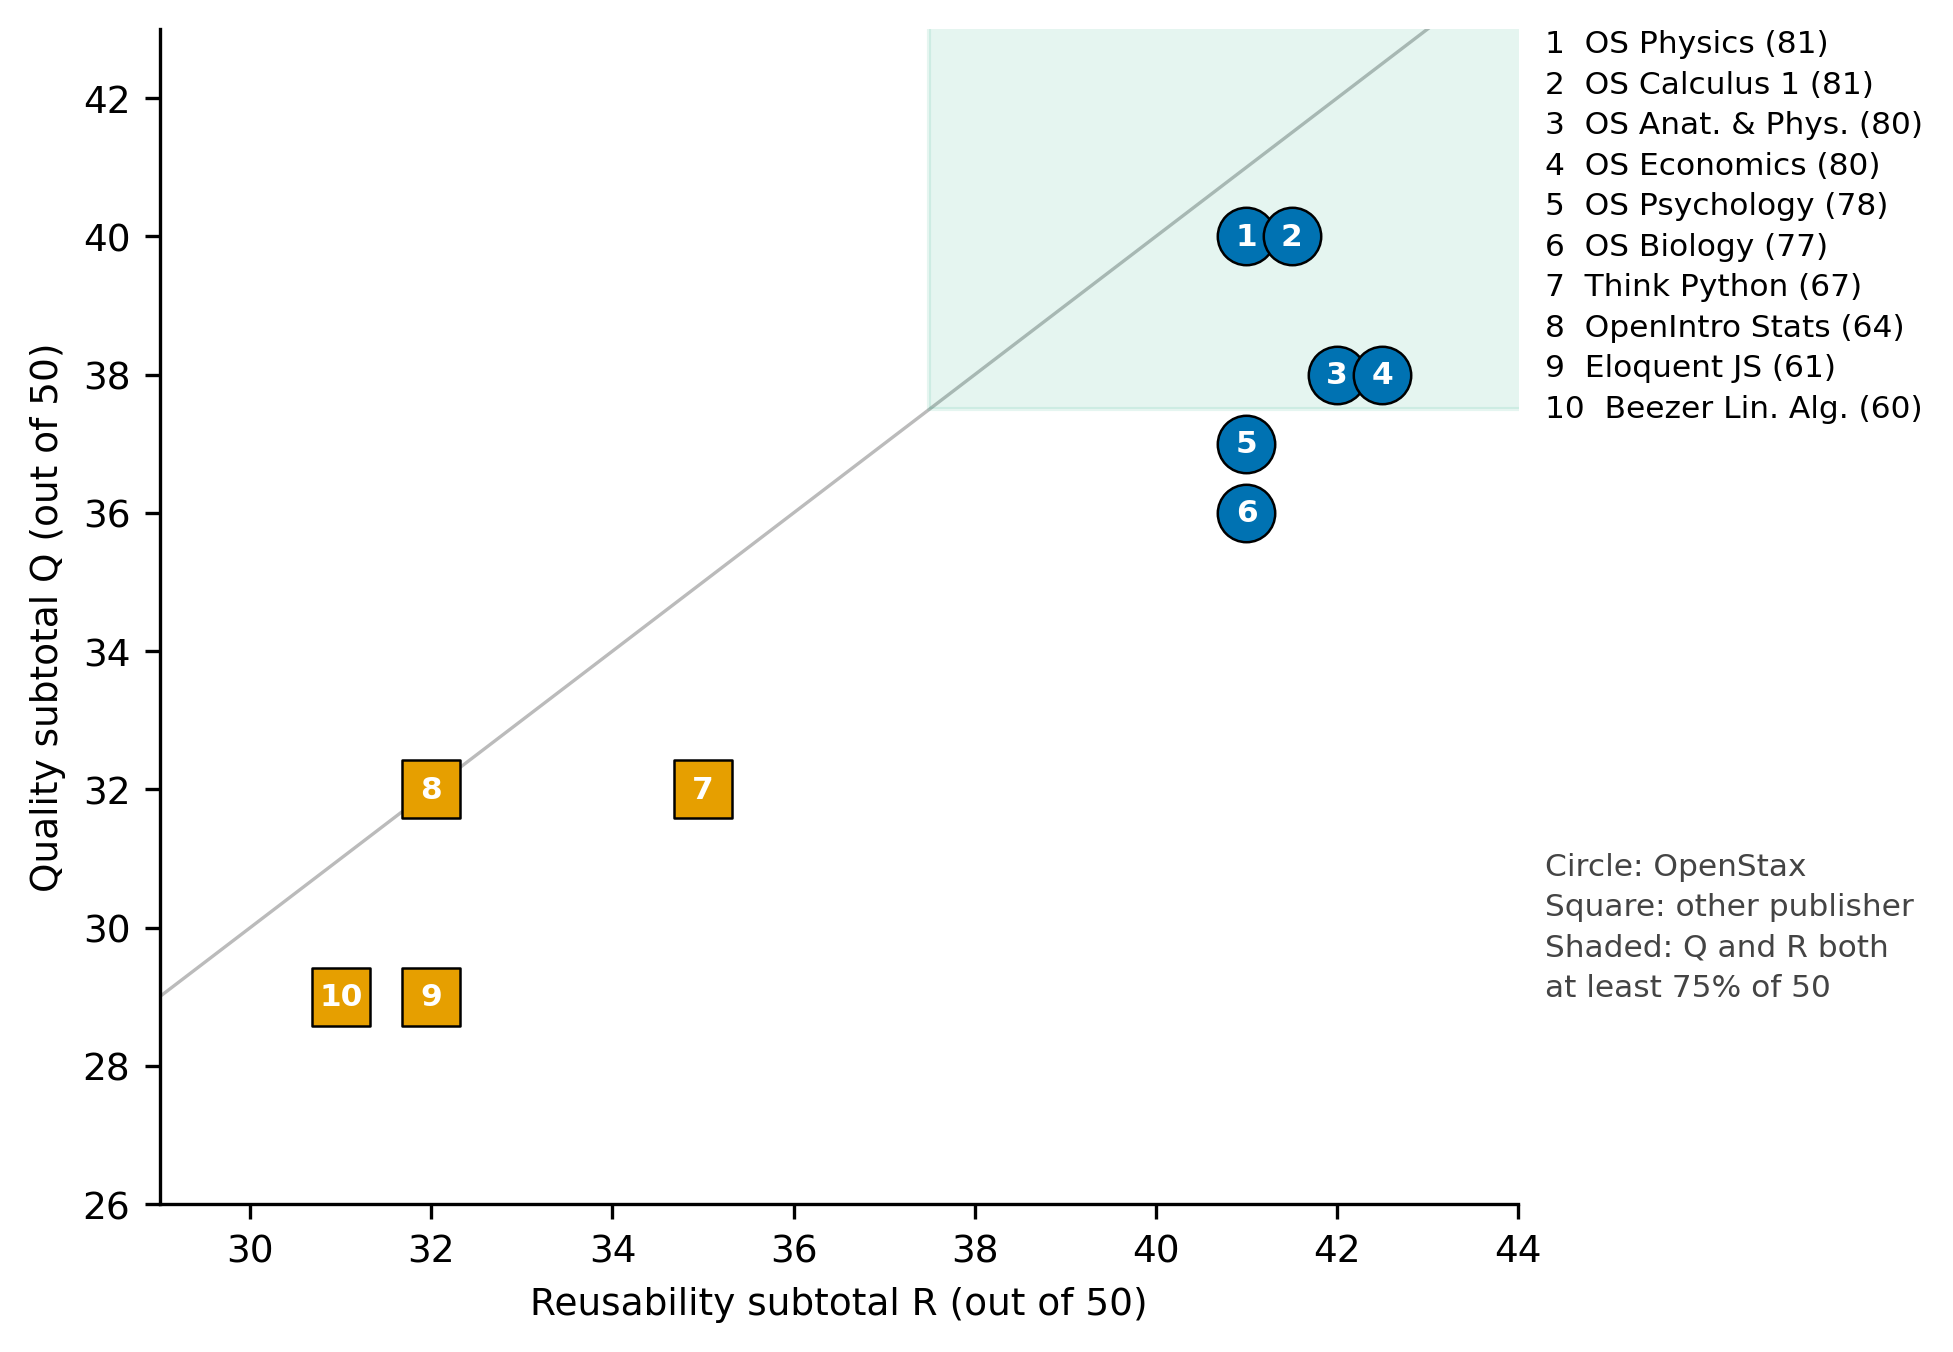
\includegraphics[width=0.92\textwidth]{figures/qr-scatter.png}
  \caption{Quality subtotal Q against reusability subtotal R for the ten scored textbooks (three-chapter pass), numbered by total score with a key at right. Every title sits on or below the diagonal, so reusability is at least as strong as quality for all ten. The four titles in the shaded region have both subtotals at least 75 percent of 50. Points with identical Q and R are offset slightly so both remain visible.}
  \label{fig:qr}
\end{figure}

\begin{figure}[htbp]
  \centering
  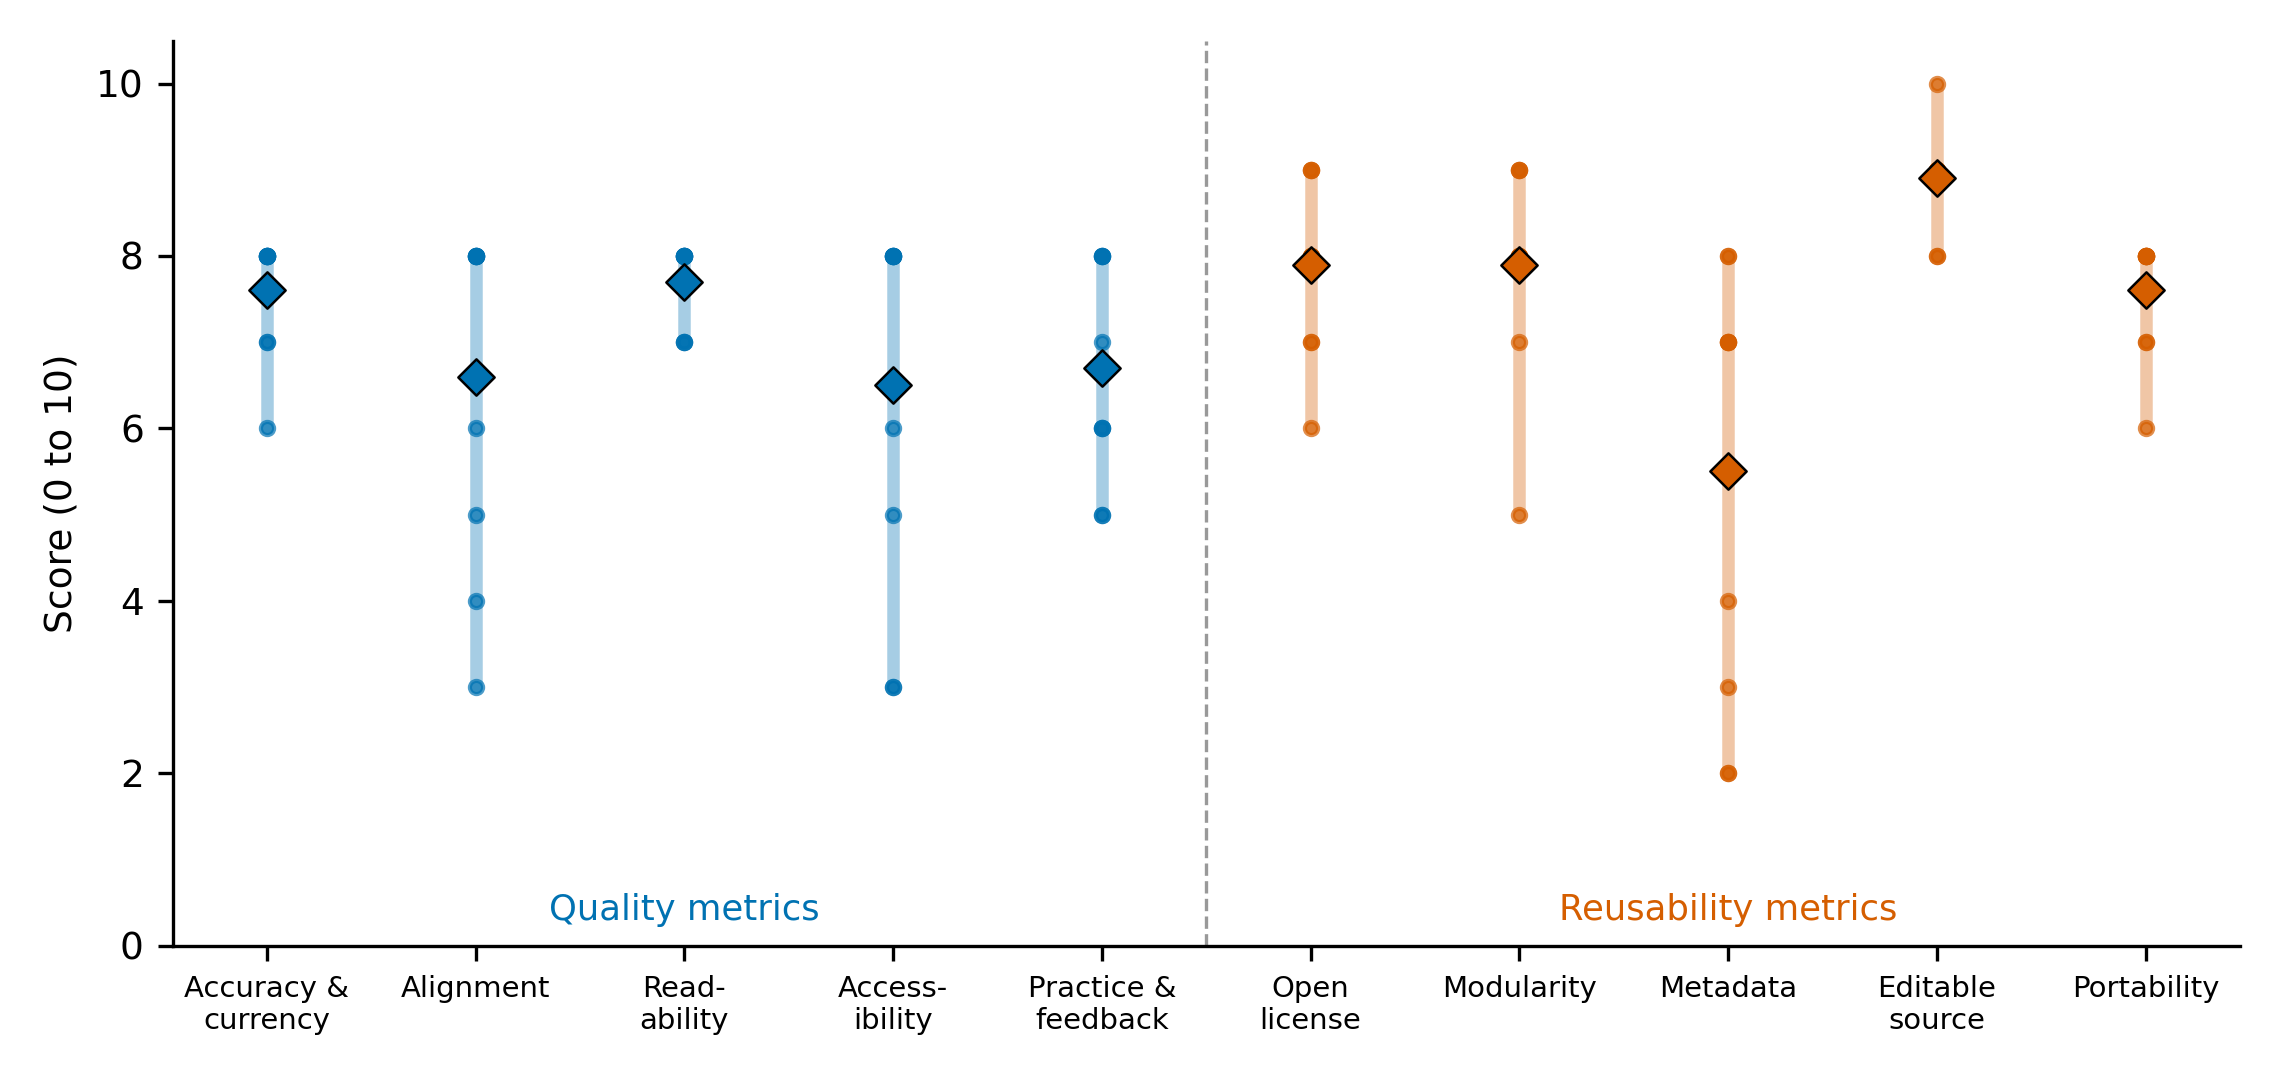
\includegraphics[width=0.95\textwidth]{figures/metric-profile.png}
  \caption{Score distribution for each of the ten metrics across the ten textbooks (three-chapter pass): individual scores (dots), range (bar) and mean (diamond), with quality metrics in blue and reusability metrics in vermilion. Metadata has the lowest mean and the widest spread among reusability metrics; accessibility and alignment have the widest spread among quality metrics.}
  \label{fig:profile}
\end{figure}

\subsection{What the scores surface}
\paragraph{Reusability is at least as strong as quality.}
In the second pass R is at least Q for all ten titles, by 0 to 5 points (mean R 37.8, mean Q 35.1). A plausible reading is that content quality is simply harder to verify from public pages than a license or a source repository, so reviewers score the quality metrics conservatively; another is that open-textbook projects invest heavily in packaging. The data cannot separate these explanations. They do show why the two halves need to be reported separately: a single total of 67 for \emph{Think Python} hides that its editable-source score is the maximum (10) while its alignment and accessibility scores are only 5 and 5.

\paragraph{Metadata is the weakest metric.}
Metadata has the lowest mean (5.5) and ranges from 2 to 8. Reviewers repeatedly found descriptive and citation tags in page source but no structured educational metadata such as subject and level, or machine-readable license fields, and they found blank metadata in the one PDF-only book. This echoes the long-standing emphasis on metadata quality in learning-object repositories \cite{ochoa2009}.

\paragraph{Editable source is the strongest.}
Editable source has the highest mean (8.9, range 8 to 10), consistent with open-textbook projects publishing source on public hosting sites. Learning-outcome alignment (mean 6.6, range 3 to 8) and accessibility (mean 6.5, range 3 to 8) show the widest spread among quality metrics. For three titles (Think Python, Eloquent JavaScript, Beezer) the reviewers found no clear per-section learning outcomes. For OpenIntro Statistics, the second-pass reviewer found that the book's ``screen-reader'' PDF is marked untagged and that no alternative text appeared in its extracted text, which the first-pass reviewer could not check.

\paragraph{Licenses: eight of ten carry a NonCommercial term, and the rubric is under-specified.}
The six OpenStax titles and \emph{Think Python} are CC BY-NC-SA 4.0, and \emph{Eloquent JavaScript} is CC BY-NC 3.0; OpenIntro is CC BY-SA 3.0 and Beezer's text is under the GNU Free Documentation License. No title is CC BY. The license metric scored 8 or 9 for the six NC-SA OpenStax titles, 7 for \emph{Think Python} (also NC-SA) and 6 for \emph{Eloquent JavaScript}. Reviewers described weighing the NonCommercial term, the license version, third-party notices and whether a license line appears on every page, and they weighed them differently; the descriptors of Table~\ref{tab:bands} do not say how a restrictive-but-clear license should be scored. This is the kind of under-specification an anchored rubric must remove (R1).

\paragraph{Agents report their own uncertainty.}
Each agent listed between 6 and 8 things it could not verify, such as whether a license notice appears on every page, whether LMS packages import cleanly, and whether alternative text is meaningful. These statements are useful, but they are self-reports and have not been checked against an independent reviewer.

\subsection{Stability across the two passes}
\label{sec:retest}
The first pass (one chapter) and second pass (three chapters) are independent applications of the same instrument by different agents of the same model family. Comparing them gives a first, rough estimate of how stable scores are; Figure~\ref{fig:passes} plots the totals.

\begin{figure}[htbp]
  \centering
  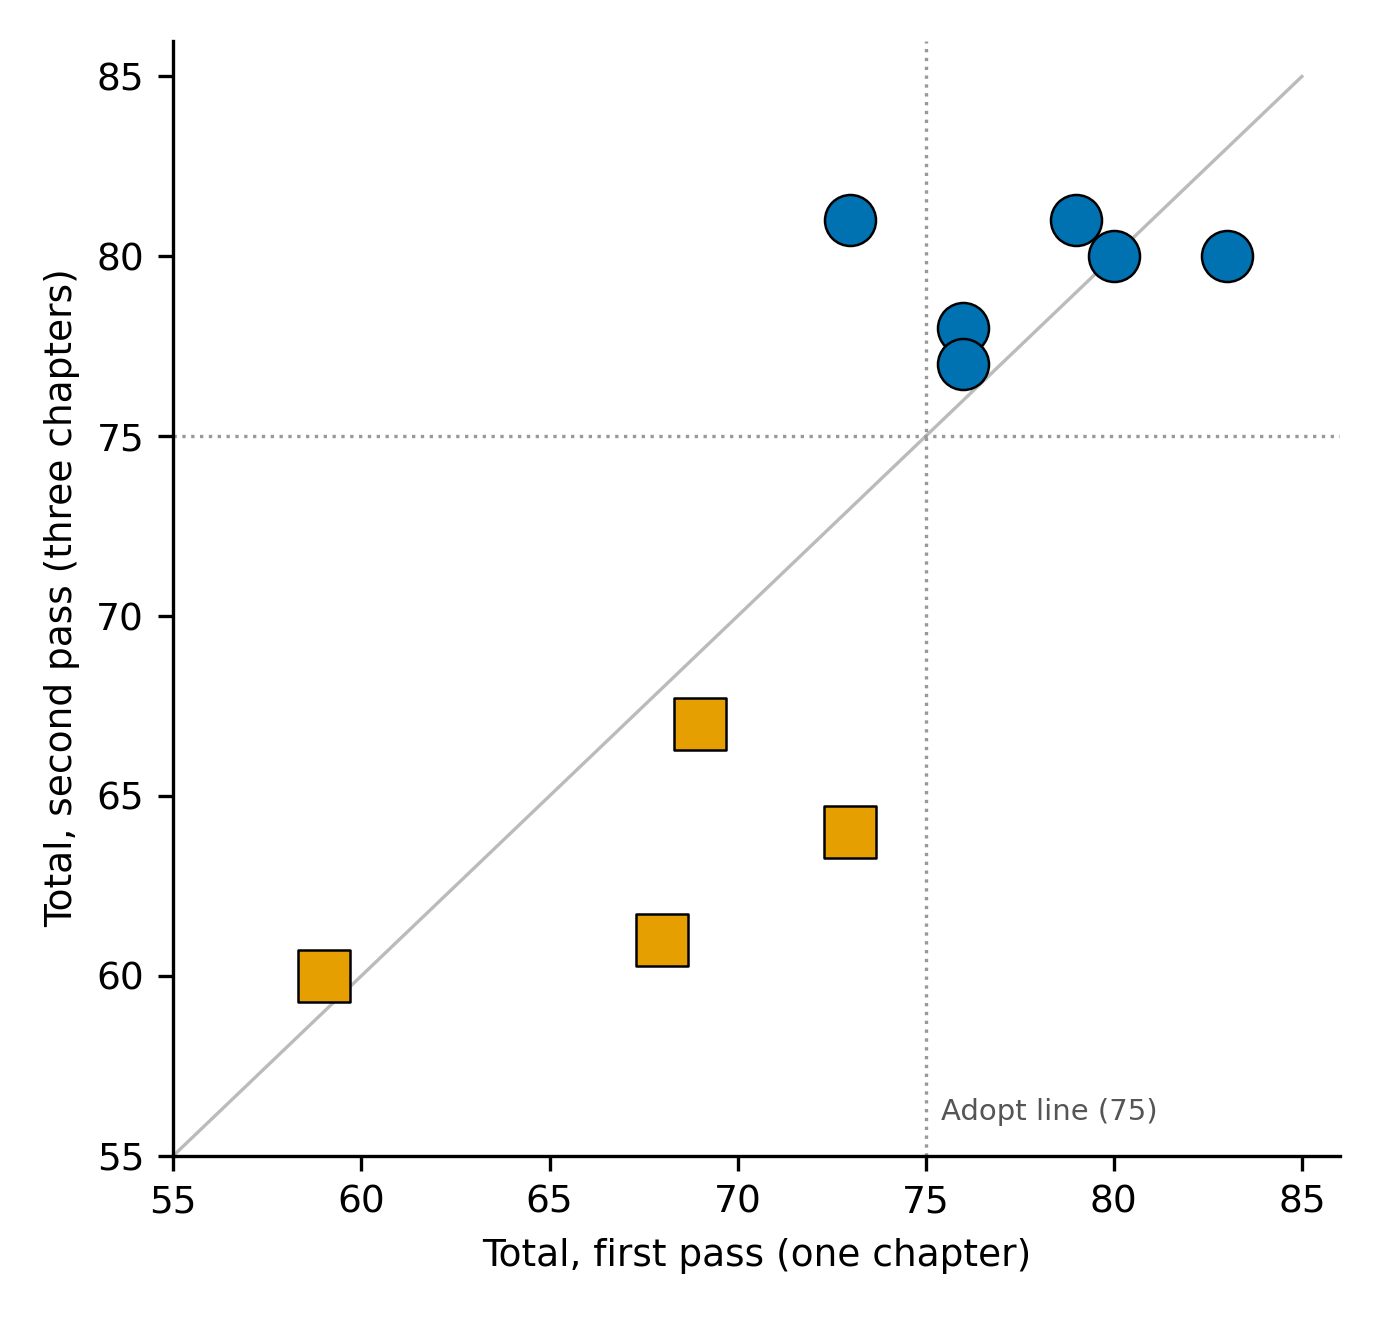
\includegraphics[width=0.62\textwidth]{figures/passes-scatter.png}
  \caption{Total score from the first, one-chapter pass (horizontal) against the second, three-chapter pass (vertical) for the ten textbooks; circles are OpenStax titles and squares are other publishers. Points near the diagonal were scored alike; the dotted lines mark the Adopt threshold of 75. One title (Calculus Volume 1) crosses the threshold between passes and the other nine keep their decision.}
  \label{fig:passes}
\end{figure}

Totals differ by a mean of 3.5 points between passes (rank correlation 0.75), and nine of the ten decisions are unchanged; Calculus Volume 1 moves from Revise (73) to Adopt (81). Across the 100 metric scores, the two passes agree exactly 46 percent of the time and within one point 88 percent of the time, with a quadratic-weighted kappa of 0.80 \cite{cohen1960,landis1977}. For the five reusability metrics, which both passes scored from the whole work, exact agreement is 44 percent, agreement within one point is 90 percent and the weighted kappa is 0.86. For the five quality metrics, where the sampled chapters also changed, the figures are 48 percent, 86 percent and 0.71.

Three caveats apply. The kappa pools all ten metrics, so it partly reflects differences between books; with ten books we cannot estimate it per metric. Both passes used the same model family and the same brief, so their errors may be correlated, and this agreement is probably an upper bound on what independent human reviewers would achieve. And because the reviewer and the sampled chapters changed together for metrics 1 to 5, the comparison cannot separate reviewer noise from chapter effects there. The reusability metrics isolate reviewer noise, and their mean absolute difference (0.66 points) is similar to that for the quality metrics (0.72), which suggests that chapter choice adds little beyond reviewer noise for most metrics. The exception is practice with feedback: it has the lowest exact agreement (2 of 10) and the largest mean difference (1.4 points), and its per-chapter scores vary the most within a book (mean range 1.3 points, up to 6). In \emph{Think Python}, the first and middle chapters score 8 while the final reflective chapter, which has no exercises, scores 2.

Chapter choice matters most where chapters differ in kind. Across the ten books the per-chapter quality subtotal (out of 50) ranged by a mean of 2.5 points between a book's best and worst sampled chapter, but by 8 for \emph{Think Python} and 6 for OpenStax College Physics, whose final chapters are short or conceptual. A one-chapter sample is therefore adequate for some books and misleading for others, and a reviewer cannot tell in advance which.

\subsection{Cost of scoring}
Table~\ref{tab:cost} reports what scoring cost. The first pass used 827{,}549 tokens and 135 tool calls and took about 2 minutes 25 seconds of wall-clock time with ten agents in parallel. The three-chapter pass used 860{,}984 tokens and 176 tool calls and took about 3 minutes 37 seconds. Per title, the second pass took a mean of about 86{,}100 tokens and 121 seconds. Together the two passes used about 1.69 million tokens. Tripling the number of sampled chapters raised tokens by only 4 percent and time per title by 28 percent, because most of an agent's effort goes to whole-work checks and to locating evidence, not to reading additional chapters. Tokens used by the main session to coordinate the agents and to draft the paper are not included.

\begin{table}[htbp]
\centering
\caption{Resource cost of scoring ten textbooks, one agent per title, all run in parallel. Token counts are the totals reported by the agent harness for each agent. Cost is for one reviewer pass and does not include any human checking.}
\label{tab:cost}
\small
\begin{tabular}{@{}llrrr@{}}
\toprule
Pass & Measure & Mean per title & Minimum & Maximum \\
\midrule
One chapter & Tokens used & 82{,}755 & 71{,}761 & 102{,}022 \\
 & Elapsed time (seconds) & 94 & 47 & 144 \\
 & Tool calls & 13.5 & 6 & 21 \\
\addlinespace
Three chapters & Tokens used & 86{,}098 & 74{,}385 & 97{,}170 \\
 & Elapsed time (seconds) & 121 & 52 & 217 \\
 & Tool calls & 17.6 & 7 & 29 \\
\bottomrule
\end{tabular}
\end{table}

No book needed to be downloaded in full: agents read pages, archives and public APIs, and the working folders they used for scripts and fetched pages held about 109 MB in total (97 MB of it in one title's folder). The 101 scripted-census reports occupy about 114 MB of local JSON and digest files, and a scripted pass over a 203-component book took 2.3 seconds on the author's laptop.

\subsection{Scripted census of 101 book projects}
\label{sec:census}
The scripted checks passed on average 6.4 of 13 per book (median 6, range 3 to 10), and 32 books passed five or fewer (Figure~\ref{fig:census}). The checks that few books pass are narrow convention checks: a sponsor or publisher statement (6 of 101), a technical-requirements statement (8 of 101) and learning objectives detected by phrase matching (26 of 101). By contrast, a license, named creators and stated prerequisites were found in 94, 100 and 98 books, while image alternative text was present on every image in only 22. No book passed the internal-link check, which requires \emph{every} internal link to resolve; the median book resolved 97.9\% of its internal links. These results show that a large share of a rubric can be run across a catalog in seconds per book, and also show that strict pass rules, narrow phrase detectors and template-specific conventions produce numbers that need careful reading.

\paragraph{Sensitivity to the selection.} The headline is stable under reasonable changes to who is counted. Excluding the companion book (100 books) leaves the mean, median and range unchanged. Excluding it and nine more repositories that look like tooling, documentation or hardware projects by name (91 books; a judgment we did not verify by reading them) gives the same mean of 6.4 and median of 6. Restricting to the 61 books with a clean working tree gives a mean of 6.6 and a median of 7, with 16 passing five or fewer. Excluding the 5 books with unresolved merge conflicts (96 books) gives a mean of 6.4 and a median of 6.

\begin{figure}[htbp]
  \centering
  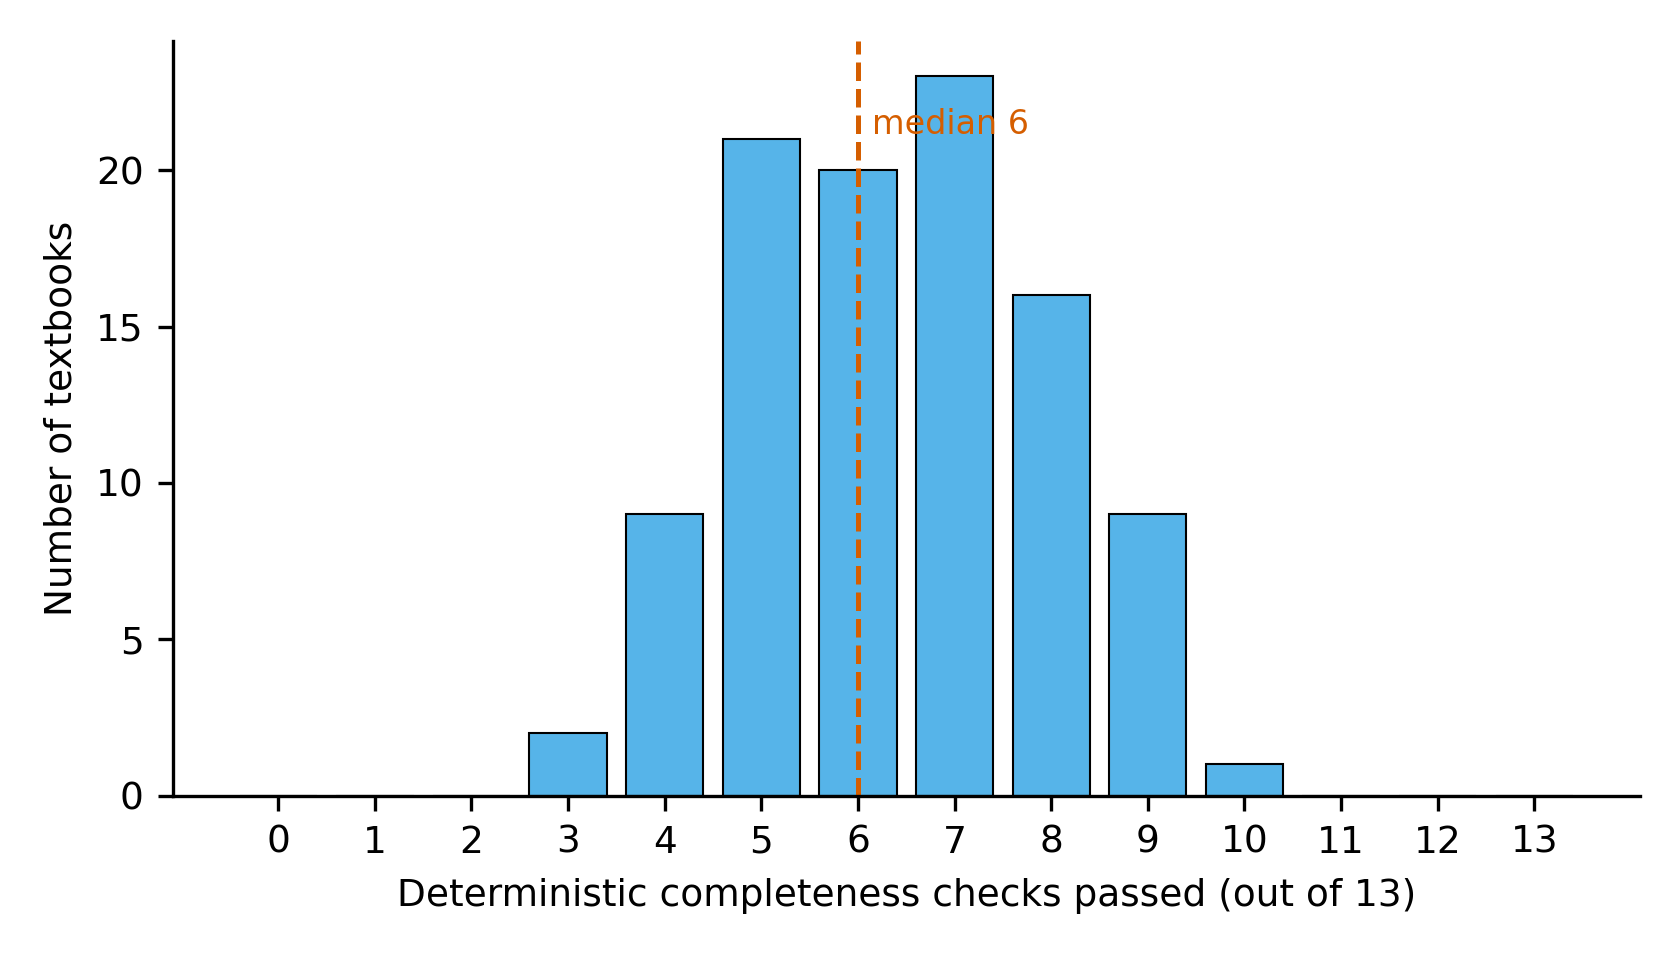
\includegraphics[width=0.78\textwidth]{figures/census-histogram.png}
  \caption{Distribution of the number of scripted completeness checks passed (out of 13) across 101 MkDocs book projects in one author's workspace. The distribution is centered near six, with a long tail of books passing few checks; only one book passes ten and none passes more. The dashed line marks the median.}
  \label{fig:census}
\end{figure}

\section{A Validation Agenda}
\label{sec:validation}

The illustration of Section~\ref{sec:illustration} shows that the instrument can be applied, not that its numbers can be trusted. We propose a sequence of studies, ordered by what each must establish before the next is worth running (R4).

\paragraph{Study 1: Descriptor refinement.}
The license finding shows that anchors are incomplete. Before any agreement study, reviewers should score a small calibration set, compare their numbers, and rewrite descriptors wherever two reviewers diverge by more than a point for reasons the text does not settle. The result is a revised, versioned rubric.

\paragraph{Study 2: Human inter-rater agreement.}
Two or more trained human reviewers score the same sample independently, with evidence recorded. Agreement per metric is reported with a chance-corrected statistic for the ordinal scores, such as a weighted kappa or Gwet's coefficient \cite{cohen1960,gwet2008}, and with an intraclass correlation for totals \cite{shrout1979,koo2016}, interpreted with stated benchmarks \cite{landis1977}. Metrics that fail to reach a pre-registered threshold are rewritten or dropped. Numbers should be reported per metric, because a high total agreement can mask one unreliable metric.

\paragraph{Study 3: Agent-versus-human agreement.}
Agent scores are compared with the human consensus on the same sample. The illustration of Section~\ref{sec:retest} is a first, weak step: two agent passes agreed within one point on 88 percent of metric scores, but that says nothing yet about agreement with people. The analysis should report agreement per metric, systematic bias (does the agent score high?), and failure types: invented citations, misread licenses and overconfident scores \cite{ji2023}. Judge-specific biases such as position and verbosity effects \cite{zheng2023,wang2024} should be tested by perturbing the order and length of inputs. Agreement must be reported separately for scripted checks and for judgment checks, so that error is attributed correctly.

\paragraph{Study 4: Construct validity.}
Do scores measure what the metrics name? Methods include comparison with existing rubrics applied to the same resources \cite{yuan2015}, convergent checks against independent measures (for example an accessibility audit against metric 4, or a metadata-completeness measure \cite{ochoa2009} against metric 8), and expert review of whether the ten metrics cover the constructs adopters care about.

\paragraph{Study 5: Predictive validity.}
Does a higher score predict better outcomes? The strongest test is a controlled comparison in which students use an original resource and an improved version whose score is higher, with learning measured on a common assessment. Studies of OER efficacy show that the relationship between OER and learning is itself unsettled \cite{tlili2023,hilton2020}, so this study is likely to find that some metrics predict outcomes and others do not. That would be a useful result: it tells adopters which metrics matter for learning and which matter for reuse only.

\paragraph{Study 6: Consequences and gaming.}
Once a score guides adoption, authors will optimize for it \cite{campbell1979,strathern1997}. Authors can add metadata fields and alternative text cheaply; they cannot as cheaply make facts accurate. The program should monitor whether score gains from cheap-to-game metrics outpace score gains from costly ones, and whether the rubric should audit evidence by sampling.

\paragraph{Reporting.}
Every score published before Studies 2 and 3 are complete should carry a ``provisional'' label. Studies and their data should be public, versioned and replicable, so that the rubric can be revised openly and its history inspected.

\section{Discussion and Limitations}
\label{sec:discussion}

\subsection{Implications}
\paragraph{For adopters.} A QR report is best read as a structured screening aid with an evidence trail, not as a verdict. The split into Q and R tells an instructor whether a weak resource needs better content or better packaging, and the per-metric evidence shows where to look. The illustration suggests that even widely used titles leave room to improve: no scored title reached the excellent band, and the Adopt decision for five titles depends on the floor rule of Equation~\ref{eq:decision} as much as on the total.

\paragraph{For authors and publishers.} Several of the weakest scores are cheap to fix. Metadata was the weakest metric in the illustration, and structured descriptive and license metadata can be added without changing a word of content. Stated learning outcomes and accessibility statements are the next most tractable. The score thus points to specific, ordered improvements, which is what makes it more useful than a star rating.

\paragraph{For repositories and policy.} A catalog that published the ten scores, with evidence and version, alongside each record would let users filter on the properties they care about. A shared instrument also gives policy bodies something to measure progress against, which a recommendation alone does not provide \cite{unesco2019}.

\paragraph{For researchers.} The program in Section~\ref{sec:validation} treats rubric design as an empirical problem, as the review of existing rubrics urges \cite{yuan2015}. The most informative findings may be negative: metrics that do not agree across reviewers, or that do not predict learning.

\subsection{Limitations}
\begin{itemize}[leftmargin=*,itemsep=3pt]
  \item \textbf{One model family, no human reviewer.} Each title was scored in two passes by AI agents of the same model family, with no human scoring the same resource. The scores can carry that model's biases, and the two passes may share errors, so the agreement between them is probably an upper bound on human agreement. With ten titles we cannot estimate agreement per metric. The scores are therefore illustrations of the instrument, not measurements of the books.
  \item \textbf{Sampling.} Metrics 1 to 5 were scored from three chapters per book (first, middle and last numbered). The first pass used a single chapter, and its totals differed from the three-chapter totals by 3.5 points on average and by 9 for one title. Three chapters is still a small sample of a book with 16 to 47 chapters, and the first-pass rule (the fifth chapter) was itself ambiguous for a book with an unnumbered introduction.
  \item \textbf{Convenience sample.} The ten books were chosen by judgment, include six from one publisher, and are all in STEM or social-science introductory subjects with English text. The sample cannot support claims about OER in general.
  \item \textbf{Limited access for the reviewer.} Agents could read pages and public APIs but did not render pages in a screen reader, test contrast, import LMS packages or check every page for a license line. Some pages (for example a publisher's accessibility statement) were not readable without a script engine. Each agent listed what it could not verify, and its confidence labels are self-reports. In the first pass one agent reported that a shared working folder was overwritten by another agent and re-fetched its files; we have not checked whether this affected its readings, and in the second pass each agent had its own folder.
  \item \textbf{Scripted census scope.} The 101-book census is the author's own corpus of MkDocs textbooks, mostly generated by one pipeline, and the checks encode that pipeline's conventions (for example, phrase detection for learning objectives). The low pass rates for some checks say more about convention-matching than about the books.
  \item \textbf{Equal weights and a total.} Equal weights are a default, not a finding. The companion component-level specification keeps its two headline numbers separate on purpose \cite{oerevaluator}, whereas the QR report adds them; whether a combined total helps or misleads adopters is untested.
  \item \textbf{Author's interest.} The author wrote the rubric, the companion book and the evaluator skill, which is a conflict of interest for any claim that the instrument works. The independent studies of Section~\ref{sec:validation} are the remedy. The name ``OpenBook'' has not been searched for conflicts with existing marks or projects.
  \item \textbf{Not a learning measure.} The score examines the resource, not its effect on learners, and it is a snapshot of one date, 31 October 2026.
\end{itemize}

\subsection{Open design questions}
The illustration points to questions the specification should settle before validation. Should a NonCommercial or share-alike clause cap the license metric at a stated number? Should scripted checks determine fixed shares of some metrics, so that agents can no longer drift on them? Should a resource that fails a floor metric be reported with a warning flag even when its total is high? Each is an empirical question for Studies 1 and 2.

\section{Next Step: Verifying Chapter Content with a Low-Cost Model}
\label{sec:nextstep}

The work reported here is a \emph{fast, low-cost first step}. It samples three chapters per book, reads public pages and repositories, and scores structural indicators of quality and reusability in minutes. Its main weakness is on the quality side: no reviewer checked whether the content of a chapter is correct. The metric called accuracy and currency is in practice a proxy (an errata process, a recent revision), and alignment, readability and practice are judged from page structure. The next step, planned for a future paper, adds claim-level verification of sample chapters using a small, low-cost language model, Claude Haiku, as a flagger inside a pipeline in which code does everything that can be exact. We describe the design here so that it can be criticized before it is run. \emph{No results are reported, and how well such a pipeline works is unknown.}

\subsection{Design}
\begin{enumerate}[leftmargin=*,itemsep=2pt]
  \item \textbf{Split the work.} Code handles what can be exact: splitting a chapter into sections, reading level, image and alternative-text counts, and parsing exercises and answers. The model handles small, bounded language tasks and returns structured output with exact quotations and sentence identifiers.
  \item \textbf{Ground every judgment in evidence.} The model never judges a claim from memory. It is given the cited source or retrieved snippets and must quote the passage it relies on; code checks that the quotation appears verbatim in the chapter or source, which catches invented evidence. A claim with no retrievable evidence is recorded as unverifiable, not as true.
  \item \textbf{Repeat and compare.} Each judgment is made three times with the order of inputs shuffled and the prompt reworded. Disagreement is kept as an uncertainty flag, not averaged away.
  \item \textbf{Calibrate before trusting.} The pipeline is first run on a chapter seeded with known errors (a wrong value, a swapped definition, a citation that does not support its claim, an exercise that matches no objective). Its detection rate and false-alarm rate on those errors are reported before it is applied to any real chapter.
  \item \textbf{Escalate.} Only flagged items go to a stronger model, and disputed items go to a human reviewer.
  \item \textbf{Report, do not score.} The output is a verification report, for example the numbers of supported, contradicted, unsupported and unverifiable claims with their quotations. It would anchor the accuracy metric to a share of verified claims and leave unverifiable items marked as insufficient evidence.
\end{enumerate}

\begin{table}[htbp]
\centering
\caption{Planned tasks for the low-cost model on one sample chapter, and the exact check that code applies to each output. The pipeline has not yet been run.}
\label{tab:nextstep}
\small
\begin{tabular}{@{}L{3.0cm}L{5.8cm}L{5.0cm}@{}}
\toprule
Task & What the model does & Check applied by code \\
\midrule
Claim extraction & Lists the checkable factual claims in a section, each with a sentence identifier. & Every quotation must appear verbatim in the chapter. \\
Citation support & Given a claim and the text of its cited source, answers supported, contradicted or not addressed, with the supporting passage. & The passage must appear verbatim in the fetched source. \\
Uncited claims & Judges each claim against retrieved snippets, never from memory, as stable, time-sensitive or doubtful. & Snippets are logged; claims with no evidence are marked unverifiable. \\
Alignment & Maps each exercise to a stated learning objective and labels its Bloom level. & Counts objectives with no exercise and exercises with no objective. \\
Terms before definition & Lists terms a first-time reader would not know and where each first appears. & Compares each term with the glossary and the chapter text. \\
Alternative text & Given the image, caption and nearby text, says whether the alternative text describes the image. & Presence of alternative text is already counted exactly. \\
\bottomrule
\end{tabular}
\end{table}

\subsection{Evaluating the pipeline itself}
The seeded-error chapter gives measurable quantities: the share of planted errors detected, the share of flags that are false alarms, the agreement across the three repeated runs, and the tokens and time used, which can be compared with the cost of the first step in Table~\ref{tab:cost}. A pipeline that misses many planted errors, or that agrees with the book whatever it says, is not suitable as a verifier and the results would say so.

\subsection{Expected limits}
A small model can share a book's misconceptions, can be inclined to agree with text it is shown, and may miss errors in specialist domains such as mathematical proofs. It can verify only what retrieval can reach, so its recall is unknown until the seeded-error test measures it. And verifying claims does not show that a chapter teaches well; that remains the question for the learner-outcome studies of Section~\ref{sec:validation}.

\section{Conclusion and Future Work}
\label{sec:conclusion}

\paragraph{This is a first step.}
This paper does not validate the OpenBook QR Score, and its scores should not be read as measurements of how good or how reusable the ten textbooks are. It is a fast, low-cost first step: an argument for what an objective OER score must be, a specification of one candidate, and an illustration that applies the candidate to ten books in minutes of wall-clock time per pass. Every score comes from AI agents of one model family, from three sampled chapters per book, and no human reviewed any resource.

\paragraph{What the first step showed.}
We argued that deciding which open educational resources to adopt needs a shared instrument that is anchored, two-part, reproducible and validated, and that existing rubrics, as surveyed in the literature, meet these requirements only partly. We proposed the OpenBook QR Score, a ten-metric, 100-point instrument whose report keeps quality and reusability visible as QR 76 (Q 37 / R 39) and whose decision rule guards against a high total hiding a failed metric. The illustration showed the instrument's value (it points to concrete fixes, and two passes agreed within one point on 88 percent of metric scores) and its weaknesses (descriptors for restrictive licenses are loose, practice with feedback is unstable across chapters, and quality is judged mainly from structure, not from checked content).

\paragraph{The next step.}
The next step, for a future paper, is to verify the content of sample chapters with a low-cost model, Claude Haiku, in the evidence-grounded, repeated and calibrated pipeline of Section~\ref{sec:nextstep}. It targets the weakest part of this paper, the accuracy of the quality metrics, and it will be tested first on chapters seeded with known errors.

\paragraph{The steps after that.}
Four further steps follow. First, tighten the descriptors where the illustration exposed drift, starting with licenses and learning outcomes. Second, run the human and agent agreement studies of Section~\ref{sec:validation}, with at least two independent human reviewers per resource and several chapters per book. Third, test whether scores predict learner outcomes in controlled comparisons of an original resource and an improved version. Fourth, publish scores with their evidence and version in an open catalog, so that the community can dispute and improve them. Until those steps are done, every OpenBook QR Score should be labeled provisional.


\section*{Acknowledgments}
The ten-metric rubric builds on the review of OER quality rubrics by Yuan and Recker, whose
article is published under a CC BY 4.0 license. The OpenStax, OpenIntro, Green Tea Press and
other open textbook authors whose books are scored in Section~\ref{sec:illustration} made
that illustration possible; the scores describe the scoring method, not the quality of those
authors' work.

\paragraph{Use of generative AI.}
Claude (Anthropic; Sonnet 5.5 through the Claude Code agent harness) was used to draft the
text from the author's repository and notes, to write the figure scripts, to run the scripted
checks, and to format references. Twenty Claude agent runs (ten textbooks in each of two passes) applied the rubric in
Section~\ref{sec:illustration}; their output is reported as data and is not independent
expert review. Every reference was checked against Crossref or the publisher's page. The author
reviewed, edited and takes full responsibility for the content.

% References
\bibliographystyle{ieeetr}
\bibliography{sections/references}

\end{document}
